% Options for packages loaded elsewhere
\PassOptionsToPackage{unicode}{hyperref}
\PassOptionsToPackage{hyphens}{url}
\PassOptionsToPackage{dvipsnames,svgnames*,x11names*}{xcolor}
%
\documentclass[
  12pt,
]{article}
\usepackage{lmodern}
\usepackage{setspace}
\usepackage{amssymb,amsmath}
\usepackage{ifxetex,ifluatex}
\ifnum 0\ifxetex 1\fi\ifluatex 1\fi=0 % if pdftex
  \usepackage[T1]{fontenc}
  \usepackage[utf8]{inputenc}
  \usepackage{textcomp} % provide euro and other symbols
\else % if luatex or xetex
  \usepackage{unicode-math}
  \defaultfontfeatures{Scale=MatchLowercase}
  \defaultfontfeatures[\rmfamily]{Ligatures=TeX,Scale=1}
  \setmainfont[]{Times New Roman}
  \setsansfont[]{Times New Roman}
\fi
% Use upquote if available, for straight quotes in verbatim environments
\IfFileExists{upquote.sty}{\usepackage{upquote}}{}
\IfFileExists{microtype.sty}{% use microtype if available
  \usepackage[]{microtype}
  \UseMicrotypeSet[protrusion]{basicmath} % disable protrusion for tt fonts
}{}
\makeatletter
\@ifundefined{KOMAClassName}{% if non-KOMA class
  \IfFileExists{parskip.sty}{%
    \usepackage{parskip}
  }{% else
    \setlength{\parindent}{0pt}
    \setlength{\parskip}{6pt plus 2pt minus 1pt}}
}{% if KOMA class
  \KOMAoptions{parskip=half}}
\makeatother
\usepackage{xcolor}
\IfFileExists{xurl.sty}{\usepackage{xurl}}{} % add URL line breaks if available
\IfFileExists{bookmark.sty}{\usepackage{bookmark}}{\usepackage{hyperref}}
\hypersetup{
  colorlinks=true,
  linkcolor=Maroon,
  filecolor=Maroon,
  citecolor=Blue,
  urlcolor=Blue,
  pdfcreator={LaTeX via pandoc}}
\urlstyle{same} % disable monospaced font for URLs
\usepackage[margin=1in]{geometry}
\usepackage{longtable,booktabs}
% Correct order of tables after \paragraph or \subparagraph
\usepackage{etoolbox}
\makeatletter
\patchcmd\longtable{\par}{\if@noskipsec\mbox{}\fi\par}{}{}
\makeatother
% Allow footnotes in longtable head/foot
\IfFileExists{footnotehyper.sty}{\usepackage{footnotehyper}}{\usepackage{footnote}}
\makesavenoteenv{longtable}
\usepackage{graphicx,grffile}
\makeatletter
\def\maxwidth{\ifdim\Gin@nat@width>\linewidth\linewidth\else\Gin@nat@width\fi}
\def\maxheight{\ifdim\Gin@nat@height>\textheight\textheight\else\Gin@nat@height\fi}
\makeatother
% Scale images if necessary, so that they will not overflow the page
% margins by default, and it is still possible to overwrite the defaults
% using explicit options in \includegraphics[width, height, ...]{}
\setkeys{Gin}{width=\maxwidth,height=\maxheight,keepaspectratio}
% Set default figure placement to htbp
\makeatletter
\def\fps@figure{htbp}
\makeatother
\setlength{\emergencystretch}{3em} % prevent overfull lines
\providecommand{\tightlist}{%
  \setlength{\itemsep}{0pt}\setlength{\parskip}{0pt}}
\setcounter{secnumdepth}{5}
\usepackage{booktabs}
\usepackage{longtable}
\usepackage{array}
\usepackage{multirow}
\usepackage{wrapfig}
\usepackage{float}
\usepackage{colortbl}
\usepackage{pdflscape}
\usepackage{tabu}
\usepackage{threeparttable}
\usepackage{threeparttablex}
\usepackage[normalem]{ulem}
\usepackage{makecell}
\usepackage{xcolor}

\title{\vspace{1cm}Preaching to Social Media: Turkey's Friday Khutbas and Their Effects on Twitter\footnote{Corresponding address: \href{mailto:ozan.aksoy@ucl.ac.uk}{\nolinkurl{ozan.aksoy@ucl.ac.uk}}, 55-59 Gordon Square, WC1H 0NU, London UK. Acknowledgments: This project is funded by the British Academy through Small Research Grant no SRG20\textbackslash200045. The article is written using the R Markdown template provided by Bauer (\protect\hyperlink{ref-bauer2020writing}{2020}). David Schoch is acknowledged for sharing their \href{https://gist.github.com/schochastics/1ff42c0211916d73fc98ba8ad0dcb261}{code} for Academic Twitter. Part of the data comprises the full archive of tweets on selected topics which Twitter generously gave access to. This research obtained approval from the UCL IoE ethics panel (application no: REC1432). All analysis code are available at: link-to-be-inserted. }\vspace{0.5cm}\\}
\author{Ozan Aksoy\\
Centre for Quantitative Social Science,\\
UCL Social Research Institute\\
University College London}
\date{First version: May 11, 2021\\
This version: May 11, 2021}

\begin{document}
\maketitle
\begin{abstract}
\noindent\setstretch{1}In this study I analyse through machine learning the content of all Friday \emph{khutbas} (sermons) read to millions of citizens in thousands of Mosques of Turkey since 2015. I focus on six non-religious and recurrent topics that feature in the sermons, namely \emph{business}, \emph{family}, \emph{nationalism}, \emph{health}, \emph{trust}, and \emph{patience}. I demonstrate that the content of the sermons respond strongly to events of national importance. I then link the Friday sermons with \textasciitilde4.8 million tweets on these topics to study whether and how the content of sermons affects social media behaviour. I find generally large effects of the sermons on tweets, but there is also heterogeneity by topic. It is strongest for nationalism, patience, and health and weakest for business. Overall, these results show that religious institutions in Turkey are influential in shaping the public's social media content and that this influence is mainly prevalent on salient issues. More generally, these results show that mass offline religious activity can have strong effects on social media behavior. \newline~\newline~\textbf{Keywords:} Text-as-data analysis, computational social science, social media, religion, Islam, Turkey\vspace{.8cm}
\end{abstract}

\setstretch{1.2}
\hypertarget{introduction}{%
\section{Introduction}\label{introduction}}

On Fridays at noon Muslims hold a special mass. Practicing men are required to listen to a \emph{khutba}, a sermon delivered by the Mosque's Imam. The sermons are religious, but they often feature mundane topics. In Turkey Friday sermons are written centrally by the Presidency of Religious Affairs (TPRA). The same text is read in thousands of Mosques to millions of citizens. This gives TPRA, and through it the government a massive platform to deliver key social, political, and economic messages.

On 28.02.2020 TPRA changed the Friday sermon abruptly. The planned sermon was on how a good Muslim could legitimately earn a living. But the day before, the Turkish forces in Syria were attacked with 33 casualties. The eventual sermon was entitled ``unity and solidarity on the path for God'' featuring themes on nationalism, martyrdom, and how God would help Turkey towards victory. Likewise, in 2018 a sermon treated the evils of financial interest and another earlier one preached protecting Turkish Lira against the appreciating US Dollar. These examples suggest that sermons may respond to difficulties the government was tackling at the time.

In this study, I classify through an unsupervised machine learning technique (Welbers, Atteveldt, and Benoit \protect\hyperlink{ref-WVB17}{2017}) the content of all Friday sermons written by TPRA between January 2015 and February 2021. I focus on a selected number of non-religious and recurrent topics that emerge from the text analysis and are relevant from a sociological perspective. These topics are \emph{business}, \emph{family}, \emph{nationalism}, \emph{health}, \emph{trust}, and \emph{patience}. I then analyze whether the Friday sermons affect behavior on Twitter. In particular, I test whether and how the topic salience of the khutba in a given week affects the frequency of the tweets following the Friday prayer.

The study offers a number of contributions. Firstly, it addresses a debate about the role of politics and religion in Turkey. Since 2010 the Turkish government invests heavily in TPRA. From 2010 to 2020 TPRA's budget increased from TL2.65billion to TL11.5billion and the number of religious personnel working at TPRA increased from 80,000 to 120,000 (Aksoy and Gambetta \protect\hyperlink{ref-AG21}{2021}). Öztürk (\protect\hyperlink{ref-Ozt16}{2016}) argues that under Erdogan's AKP rule TPRA has evolved into an ideological state apparatus that imposes the political ideology of the ruling party. TPRA's arm increasingly extends beyond Turkey to the European countries where many Turks live (Öztürk and Sözeri \protect\hyperlink{ref-uxf6ztuxfcrk_suxf6zeri_2018}{2018}). It is unclear, however, if TPRA is influential in affecting public values and opinion. Despite the recent surge in TPRA's reach, religiosity seems to be in decline since 2008 (KONDA \protect\hyperlink{ref-Kon19}{2019}\protect\hyperlink{ref-Kon19}{a}). As to Khutbas specifically, a rare systematic study shows that the sermons respond to the ``threat salience'' (e.g.~frequency of terrorism-related news) (Alper et al. \protect\hyperlink{ref-alper2020changes}{2020}). Yet, the authors do not analyze the effect of sermons on public attitudes or study other more common threats the government faces (e.g.~the economy or the pandemic). The current study shows in a replicable way the extent to which Kutbas respond to politics and influence social media behaviour of Turkish citizens.

Secondly, the article makes a methodological contribution. Text-as-data methods, computational tools, and the availability of big social media data offer new opportunities to address social science questions (Lazer et al. \protect\hyperlink{ref-Lazer1060}{2020}). Such computational methods have been successfully applied to sociological questions in traditionally ``quantitative'' topics such as social networks, collective behaviour, emotions, population (Edelmann et al. \protect\hyperlink{ref-compsocsciARS20}{2020}), and with a particular focus on the Western context (Munger, Guess, and Hargittai \protect\hyperlink{ref-Munger_Guess_Hargittai_2021}{2021}). Yet, they have not been applied as extensively to topics such as religion, though fruitful applications take place in the study of culture (e.g.~Light and Odden \protect\hyperlink{ref-light2017managing}{2017}). Applying these tools to the analysis of hundreds of sermons and millions of tweets, the current study aims to push the boundary of computational social science to the study of religion and politics, in a non-Western context.

The current study also contributes to two broader sociological debates. The interplay between politics and religion has been a key subject in sociology. Tocqueville (\protect\hyperlink{ref-tocqueville2003democracy}{2003}) sees religion as one of the contributors to civic life and democracy. Likewise, Durkheim (\protect\hyperlink{ref-durkheim1965elementary}{1965}) conceives religion as a unifying force that facilitates solidarity through rituals and shared beliefs. Among all postulates formulated by classical theories, however, probably the ``opiate'' argument of Marx (\protect\hyperlink{ref-marx1970marx}{1970}) is the most well known. Marx (\protect\hyperlink{ref-marx1970marx}{1970}) argues that religion helps ease the suffering of the marginalised. In doing so, as the argument goes, religion also distracts the marginalised from engaging politically to address the underlying causes of their suffering. Empirical research tested whether religion buffers negative life events such as wars, economic shocks, discrimination, mental and physical health difficulties. The findings are mixed. Becker and Woessmann (\protect\hyperlink{ref-becker2013not}{2013}) show that improvements on material conditions do not result in secularisation, which is contrary to Marx's ``opiate'' argument. Other studies find that religion can work as social insurance against hardship, for example in case of negative life events people can turn to their religious communities for help and religious practice can indeed help alleviate suffering (Aksoy et al. \protect\hyperlink{ref-aksoy2020religiosity}{2021}; Chen \protect\hyperlink{ref-chen2010club}{2010}; Schnabel \protect\hyperlink{ref-Sch21}{2020}). The question of how politics and religion interact, thus, still stands.

Turkey offers a unique research context to help address this long standing question. The availability of all Friday sermons in Turkey and the massive social media data, together with the newly developing machine learning text analysis techniques provide opportunities to tackle this question in two novel ways. First, past empirical research mostly considers how religious individuals respond to political issues. How religious institutions respond to circumstances is relatively understudied. Second, most research is conducted in Western countries that have relatively strong democratic traditions. The interplay between politics and religion is most rife in the Middle East. The rise of political Islam in Turkey after 2002 epitomized by Erdogan's AKP (Aksoy and Billari \protect\hyperlink{ref-aksoy2018political}{2018}; Aksoy and Gambetta \protect\hyperlink{ref-AG21}{2021}) and AKP's heavy investment in the country's sole religious authority, the Turkish Presidency of Religious Affairs (Öztürk \protect\hyperlink{ref-Ozt16}{2016}; Öztürk and Sözeri \protect\hyperlink{ref-uxf6ztuxfcrk_suxf6zeri_2018}{2018}) provide a test case to understand how religious institutions respond to threats the government faces and whether these institutions' influence radiates beyond the Mosque, such as to social media, when they are backed strongly by the state.

Finally, the current study contributes to the debates on secularisation and secular transition. The secular transition model postulates a nearly universal transition as societies continue to modernise, from religious to weakly religious to nonreligious (Norris and Inglehart \protect\hyperlink{ref-norris2011sacred}{2011}; Voas \protect\hyperlink{ref-voas2009rise}{2009}). There is indeed evidence that secularisation has been taking place in many countries (Bruce \protect\hyperlink{ref-bruce2011sec}{2011}; Norris and Inglehart \protect\hyperlink{ref-norris2011sacred}{2011}; Stolz \protect\hyperlink{ref-Sto20}{2020}) and a particular debate on the United States (Schnabel and Bock \protect\hyperlink{ref-schnabel2017persistent}{2017}; Voas and Chaves \protect\hyperlink{ref-voas2016united}{2016}, \protect\hyperlink{ref-voas2018even}{2018}). Research on secularisation in non-Christian contexts, however, is relatively scarce. Being traditionally a secular country but recently embodying a rise of political Islam, the Turkish case poses an interesting challenge for this debate. On the one hand, in the last decade, as I will elaborate below there is strong and increasing government investment in religious institutions, particularly the TPRA. On the other hand, individual religiosity does not seem to have increased, in fact it seems to have decreased in the recent decades in Turkey.\footnote{See for example \href{https://www.economist.com/erasmus/2019/07/01/in-turkey-demography-is-a-brake-on-islamisation}{here} for a debate in \emph{the Economist} on government's push for Islamisation versus secularisation in Turkey.}
While testing fully the secularisation theory in Turkey is beyond the scope of the current study, understanding the extent to which TPRA influences behaviour on social media will contribute to the understanding of whether secularisation at the individual level can be reversed or slowed down through top-down investment in religious institutions.

This curious interplay between religion and politics in Turkey deserves a detailed discussion of the context, which I do next.

\hypertarget{religion-and-politics-in-turkey}{%
\section{Religion and politics in Turkey}\label{religion-and-politics-in-turkey}}

In the 2002 parliamentary elections which came in the wake of a homegrown economic crisis, a new party, AKP (Justice and Development Party--\emph{Adalet ve Kalkinma Partisi}) obtained 35 percent of the popular votes under the leadership of Recep Tayyip Erdogan and became the largest political party of the country. Due to the peculiar features of Turkey's electoral system, with only 35\% of the popular votes, AKP gained 66\% of all parliamentary seats. Since then, AKP consolidated its power. Excluding minor setbacks, AKP has won all elections since 2002 and remains the largest political party of the country to date.

The AKP has its roots in the long tradition of Turkey's political Islam (Mecham \protect\hyperlink{ref-mecham2004ashes}{2004}). The first explicitly Islamist political party of Turkey is the National Order Party (MNP) of Necmettin Erbakan which was founded in 1970 (Özbudun \protect\hyperlink{ref-ozbudun2006political}{2006}). The MNP evolved through Turkey's once staunchly secular system into the Welfare Party (RP) in 1983 after being shut down repeatedly by the constitutional court and military coups. In 1994 Recep Tayyip Erdogan was elected as Istanbul's mayor. He was the Welfare Party's candidate under Erbakan's leadership. In 1998 the then secular constitutional court shut down once again the Welfare Party for violating the \emph{laicite} principle of the constitution. Turkey's political Islam then split into two: AKP lead by Erdogan that represented then an innovationist line, and the Felicity Party (Saadet) that represented the traditionalists of the Islamist movement which was endorsed by Erbakan himself (Özbudun \protect\hyperlink{ref-ozbudun2006political}{2006}). While the Felicity Party is now on the fringe (they obtained only 1.6\% of all votes in the 2018 national elections), AKP has never looked back since.

Despite its Islamist roots, AKP started, at least for many outsiders, as a moderate party. During its first decade as the governing party, AKP was seen by many as a democratising force focused on prosperity. During this time AKP reinforced a capillary system that provided local welfare and assistance to the marginalised and the poor (Aksoy and Billari \protect\hyperlink{ref-aksoy2018political}{2018}). After a setback in the 2009 recession and then changing the constitution in the 2010 referendum, however, AKP changed course. It started curtailing Turkey's secular tradition, investing heavily in religious institutions, and deploying its capillary welfare system clientelistically (Aksoy and Gambetta \protect\hyperlink{ref-AG21}{2021}; Kuran \protect\hyperlink{ref-kuran2018islam}{2018}). In 2012 Erdogan clearly indicated raising a ``pious'' generation as a policy goal (see in Turkish \href{https://www.haberler.com/modern-dindar-bir-genclikten-bahsediyorum-3375053-haberi/}{here}).

Erdogan's aim of raising a pious generation wasn't a mere rhetoric. AKP's investment in religious institutions after 2010 can be captured by a number of key statistics. Figure \ref{fig:fig-1} shows the annual budget (in billion Turkish Liras) of and the number of personnel working for TPRA. The budget figures were obtained from the Turkish Ministry of Treasure and Finance. The annual number of personnel was extracted from TPRA's annual performance reports that are publicly available. The number of personnel includes those on long or short term contracts as included in TPRA's annual performance reports. The figure shows that the annual budget of TPRA increased around six-fold from 2006 to 2020. The number of religious personnel working at TPRA also increased strongly from 2010 (\textasciitilde84,000) to a peak in 2014 (\textasciitilde140,000). Interestingly, after peaking in 2014, the number of religious personnel decreased somewhat, but then shot up again in 2019 matching the increase in the budget.\footnote{The way TPRA reports the number of their personnel in their annual reports is inconsistent. Sometimes the number of personnel on long- and short-term contracts are reported in separate tables (in which case they are added up in Figure \ref{fig:fig-1}), other times in the same table. Sometimes TPRA seems to omit the number of personnel on short term contracts altogether. Around the key jump from 2010 to 2012, however, the reports do seem consistent, while these inconsistencies may explain the fluctuations after 2014.}

\begin{figure}

{\centering 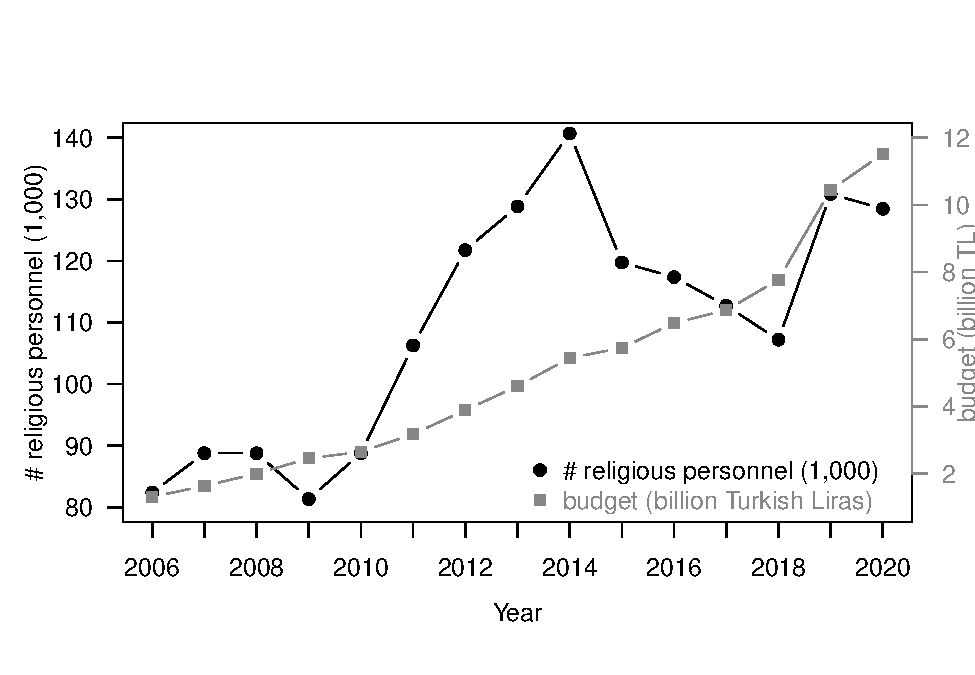
\includegraphics{Khutbas_files/figure-latex/fig-1-1} 

}

\caption{Annual budget and the number of personnel of the Turkish Presidency of Religious Affairs (TPRA) (data sources: Turkish Ministry of Treasure and Finance for budget and TPRA for personnel).}\label{fig:fig-1}
\end{figure}

A parallel ``Islamisation'' trend is also reflected in the growth of religious vocational schools (\emph{İmam-Hatip}) funded by the government. As Aksoy and Gambetta (\protect\hyperlink{ref-AG21}{2021}) report, by 2010 there were around 450 such religious secondary schools in the country, and this number was rather stable in the years before 2010. This number increased to nearly 1,500 by 2017. The annual number of students in these religious secondary schools also shot up from 12,000 in 2009 to 67,000 in 2015.

This investment in religion and TPRA has also changed TPRA's role in Turkish politics. TPRA was formed in 1924 as a ``non-political'' state institution to mainly control religion and contain the authority of local religious figures in the newly formed secular republic (Gözaydin \protect\hyperlink{ref-Guxf6zaydin2008}{2008}). Around early 1980s, TPRA has also become more active abroad in countries with large Turkish immigrant populations. After 2010, however, with the injection of public money and the government's strong support, TPRA has been transformed into a state apparatus helping implement the political ideology of AKP (Öztürk \protect\hyperlink{ref-Ozt16}{2016}). Öztürk (\protect\hyperlink{ref-Ozt16}{2016}) gives examples of this political instrumentalisation of TPRA by displaying TPRA's support for Erdogan's anti-abortion policy, pro-natalism, and deunionisation of the labour force. TPRA's foreign weight has also increased after 2010. After interviewing experts from Turkish migrant and Islamic organisations in the Netherlands and Bulgaria and reviewing TPRA's involvement in these communities, Öztürk and Sözeri (\protect\hyperlink{ref-uxf6ztuxfcrk_suxf6zeri_2018}{2018}) portray TPRA as a Turkish Foreign Policy tool with a long arm.

Overall, AKP's increasing investment in religious institutions, particularly in TPRA poses interesting questions. A number of scholars of religion have identified a widespread secularisation trend (Bruce \protect\hyperlink{ref-bruce2011sec}{2011}; Norris and Inglehart \protect\hyperlink{ref-norris2011sacred}{2011}; Stolz \protect\hyperlink{ref-Sto20}{2020}; Voas \protect\hyperlink{ref-voas2009rise}{2009}). Voas (\protect\hyperlink{ref-voas2009rise}{2009}) argues that as countries gradually modernise, they undergo a ``secular transition''
very similar to a demographic transition. The religious cohorts are gradually replaced by moderately religious (``fuzzy'') cohorts, which in turn, are replaced by the nonreligious. This model proposes the secular transition as a global pattern, but it seems to work particularly well in mostly Western countries. The increasing government investment in religion in Turkey seems to defy this secularisation trend. Yet, it is not clear if this top-down government intervention has affected much the religiosity of the citizens. While testing secularisation theory in Turkey is beyond the scope of the current study, Figure \ref{fig:fig-2} displays some motivating trends.

I use two data sources in creating Figure \ref{fig:fig-2}. The first one is Turkey's Demographic and Health Survey (TDHS) waves 2003, 2008, and 2013, which rely on representative samples of ever-married women of reproductive age (15 to 49 years) (Hacettepe University Institute of Population Studies \protect\hyperlink{ref-Hac14}{2014}).\footnote{In wave 2013, TDHS included for the first time never-married women in the sample, too, which were discarded in Figure \ref{fig:fig-2} to facilitate comparison across years.} The second dataset is extracted from the KONDA report on lifestyles in Turkey which relies on representative samples of men and women in 2008 and 2018 (KONDA \protect\hyperlink{ref-Kon19rap}{2019}\protect\hyperlink{ref-Kon19rap}{b}). Both datasets indicate a generally decreasing trend in religiosity in Turkey. In Panel A of Figure \ref{fig:fig-2} which is based on TDHS, the proportion of women who report to regulary fast and veil decreased from 86 and 71 percent, respectively in 2008, to 84 and 67 percent, respectively in 2013. In 2003, in fact, 74 percent of ever-married women reported to be veiling regularly which dropped to 67 percent in 2013.\footnote{TDHS does not ask about other religious behaviours in 2003 apart from veiling.} According to TDHS, only praying regularly seems to have gone up from 2008 to 2013 among ever-married women, from 47 percent to 51 percent. While TDHS displays only trends for ever-married women of reproductive age due to its primary sampling, the KONDA data in Panel B include both men and women of all ages. Panel B shows a remarkably similar trend of decreasing religiosity over time. For both men and women the proportion of respondents who report to sometimes, often, or always fast and pray regularly decreased from 2008 to 2018, and veiling among women decreased from 2008 to 2018. Panel B also shows that the proportion of both men and women who report to being ateists or nonreligious increased from 2008 to 2018. The decrease in religiosity among men seems to be stronger than that among women, which is relevant for the current study as only men are required to attend the Friday prayers.

\begin{figure}

{\centering 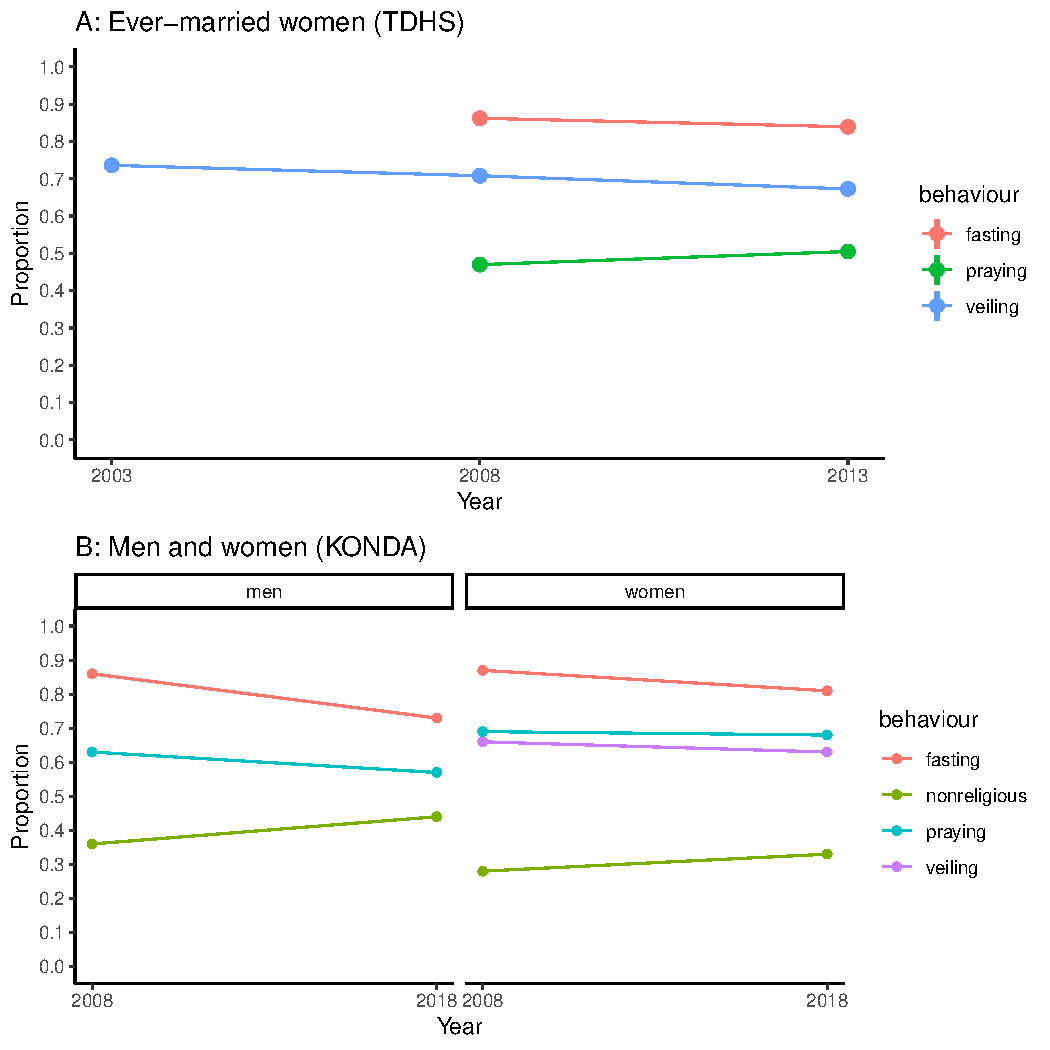
\includegraphics{Khutbas_files/figure-latex/fig-2-1} 

}

\caption{Change in indicators of religiosity. Data sources: Panel A: Turkey's Demographic and Health Survey (2003, 2008, 2013 waves, combined N = 25,226) and Panel B: KONDA life styles survey (2008 and 2018 waves, combined N = 12,275).}\label{fig:fig-2}
\end{figure}

Overall, Figure \ref{fig:fig-1} and Figure \ref{fig:fig-2} taken together pose a motivating question. While investment in TPRA has increased strongly since 2010, in keeping with the AKP's aim of ``raising pious generations'', this investment does not appear to have paid off, for religiosity at the individual level does not seem to have gone up. If anything, religiosity seems to have decreased. Does this mean that TPRA is unsuccessful in affecting public opinion and values? We cannot answer this question from Figure \ref{fig:fig-1} and Figure \ref{fig:fig-2}. This is because we don't know the counterfactual, namely, how much religiosity would have declined had the government had not invested in TPRA as much. Maybe religiosity would plummet even more without the top-down investment. To address the question as to the effectiveness of TPRA in influencing public attitudes, I turn to the question of whether Friday sermons have an effect beyond the Mosque, in the digital world.

\hypertarget{data}{%
\section{Data}\label{data}}

\hypertarget{khutbas}{%
\subsection{Khutbas}\label{khutbas}}

I scrape all khutbas that are publicly available from the TPRA website.\footnote{The archive can be reached \href{https://dinhizmetleri.diyanet.gov.tr/kategoriler/yayinlarimiz/hutbeler/hutbe-ar\%C5\%9Fivi}{here}.} I restrict the timeframe to January 2015 to Februray 2021. This is because earlier khutbas are only partially included in the TPRA archive. Moreover, the outcome variable is based on Twitter behaviour, and Twitter penetration in Turkey has plateaued in 2015 (Isman and Dagdeviren \protect\hyperlink{ref-isman2018diffusion}{2018}). Hence, the period between 2015 and 2021 provides good quality data in terms of the availability of khutbas as well as the stability of the Twitter user population in Turkey. In certain weeks when the Friday prayer coincides with the \emph{Eid}, a religious holiday, TPRA publishes two khutbas in which case the two are merged. This results in a population of 317 khutbas. Each khutba is around one to two pages of text, often stored in pdf format on the TPRA website.

\hypertarget{twitter-data}{%
\subsection{Twitter data}\label{twitter-data}}

I first analyse the khutbas with a topic modelling. Further details of the topic modelling will be presented in the next section. Here, I discuss minimal details that are relevant for Twitter data collection. After analysing the khutbas, I select six particular sermon topics and focus on them. These six topics are \emph{business}, \emph{family}, \emph{nationalism}, \emph{health}, \emph{trust}, and \emph{patience}. Each sermon topic associates with several keywords that appear in the sermon. For example, Turkish synonyms for \emph{nation}, \emph{martyr}, \emph{homeland}, and \emph{fitna} associate strongly with the topic \emph{nationalism}. I select four such keywords for each topic (see Table \ref{tab:tab1} below). I then conduct a search on Twitter's Academic Research Application Programming Interface (API) with the 24 keywords (four keywords for each of the six topics). This search is restricted to tweets tweeted from Jan-2015 to Feb-2021 (the same period as the sermons), in Turkish and from Turkey. The search returns (after nearly a week of runtime) 4,766,242 tweets which comprise the entire universe of tweets from Turkey between 2015 and February 2021 that include at least one of the 24 keywords. These tweets constitute the outcome variables in the analyses.

There are a few points worth mentioning regarding the Twitter data. Pro-government ``bots'' and ``trolls'' have been active on Turkish Twitter (Bulut and Yörük \protect\hyperlink{ref-bulut2017mediatized}{2017}). To contain the effects of these trolls and bots on the Twitter data, I exclude retweets on my search on Twitter's API. Trolls and bots mainly retweet pro-government messages. In addition, in 2020 Twitter identified 7,340 accounts from Turkey that are linked to state-backed information operations.\footnote{See for further details \href{https://blog.twitter.com/en_us/topics/company/2020/information-operations-june-2020.html}{here}.} Twitter has removed from its database these accounts and all tweets/twitter activity that are linked with these accounts. So the Twitter data collected here are free from the direct activity of these state-linked accounts. Finally, in my statistical analysis I address confounding which include possible bot/troll activity, for example, by comparing Friday pm tweets with those on Friday am in a model which also includes week ``fixed effects''.

\hypertarget{methods-and-results}{%
\section{Methods and results}\label{methods-and-results}}

\hypertarget{topic-modelling-of-khutbas}{%
\subsection{Topic modelling of Khutbas}\label{topic-modelling-of-khutbas}}

The application of machine learning to the analysis of unstructured text is becoming a powerful methodological tool for social scientists (Grimmer and Stewart \protect\hyperlink{ref-grimmer2013text}{2013}). Topic modelling, including Latent Dirichlet Allocation (LDA) and Structural Topic Models comprise a set of ``unsupervised'' machine learning tools (Blei, Ng, and Jordan \protect\hyperlink{ref-blei2003latent}{2003}; Roberts et al. \protect\hyperlink{ref-roberts2014structural}{2014}). In topic modelling, each document (in our case a khutba) is assumed to be composed of a mix of possibly many latent topics whereby each topic is associated with a set of words. The procedure then results in a word-topic matrix, similar to the matrix of the loadings of items on latent factors in exploratory factor analysis. This matrix shows how much a specific word is associated with a particular topic. The procedure also results in a topic-document matrix which reveals the extent to which a particular topic appears in a given document (i.e.~document topic probability). This process is transparent and replicable. Topic modelling, although being relatively new, has been applied to address sociological questions (Bail, Brown, and Mann \protect\hyperlink{ref-bail2017channeling}{2017}; Kennedy et al. \protect\hyperlink{ref-Racialized}{2020}; Light and Odden \protect\hyperlink{ref-light2017managing}{2017}; McFarland et al. \protect\hyperlink{ref-mcfarland2013differentiating}{2013}).

The corpus of Friday sermons comprise 317 documents corresponding to the Fridays between January 2015 and February 2021. The sermons are in Turkish. As it is common practice in quantitative text analysis, I remove words that have ignorable information content (Silge and Robinson \protect\hyperlink{ref-silge2017text}{2017}). These include common stopwords in Turkish (e.g.~synonyms for ``and'', ``but'', ``be''). I also remove words that appear in almost all sermons (e.g.~``date'', ``Ankara'', ``religious affairs'') or in almost no sermon. This results in a set of 1,139 unique words distributed across the sermons.

While there are somewhat different versions of topic modelling, I apply LDA, one of the most common topic modelling techniques (Silge and Robinson \protect\hyperlink{ref-silge2017text}{2017}). I consider models from 2 to 100 latent topics and settle on the solution with 50 topics, see also the appendix (Nikita \protect\hyperlink{ref-nikita2016select}{2016}). The exact number of latent topics in this study is not of primary importance. This is because I restrict the analysis to six particular topics, namely \emph{business}, \emph{family}, \emph{nationalism}, \emph{health}, \emph{trust}, and \emph{patience}, which appear consistently, independent of the exact number of latent topics, provided that sufficient number of topics is allowed in the model. The reason for selecting these six topics are as follows. Many topics that feature in the sermons are unsurprisingly religious and on specific theological issues, such as Ramadan fasting, life of the Prophet Muhammed, salah prayer (\emph{namaz}) etc. I am interested the extent to which TPRA affects social media behaviour in topics of sociological interest, rather than specific religious issues. For example, the topics \emph{patience} and \emph{health} and the change in their salience in the sermons over time will reveal whether and how the TPRA responds to the Covid-19 pandemic. Likewise, \emph{nationalism}, \emph{business}, and \emph{family} are key themes in the political agenda of AKP (Aksoy and Billari \protect\hyperlink{ref-aksoy2018political}{2018}). \emph{Trust} is a topic which is not normally expected to appear in a sermon but is of great interest to sociologists.

Table \ref{tab:tab1} shows the six selected sermon topics and top four terms associated with these topics that emerge as a result of the LDA. Each topic is a weighted combination of these and other words. Each sermon is, in turn, a mix of the latent topics. One of the most common topics is \emph{nationalism}. Figure \ref{fig:fig-3} shows the salience (topic probability) of nationalism in Friday sermons over time. The figure also includes a number of key dates of national importance. A date when nationalism consistently spikes in sermons is 18 March. This is what Turkey accepts as the anniversary of the Ottoman victory in the battle of Dardanelles in 1915 during the Galippoli campaign of the Entente powers in WWI. These spikes in nationalism on key dates firstly validate the LDA procedure: we find nationalism when we expect to see it. Secondly, the patterns in Figure \ref{fig:fig-3} lead to substantive findings.

\begin{table}

\caption{\label{tab:tab1}Selected sermon topics and top terms (keywords) associated with the topics. Original Turkish words are in parentheses.}
\centering
\begin{tabular}[t]{>{}lllll}
\toprule
\multicolumn{1}{c}{Topic} & \multicolumn{4}{c}{Keywords} \\
\cmidrule(l{3pt}r{3pt}){1-1} \cmidrule(l{3pt}r{3pt}){2-5}
\textbf{Health} & clean (temiz) & health (saglik) & outbreak (salgin) & caution (dikkat)\\
\textbf{Family} & family (aile) & mother (anne) & child (çocuk) & peace (huzur)\\
\textbf{Nationalism} & nation (millet) & martyr (sehit) & homeland (vatan) & fitna (fitne)\\
\textbf{Business} & forbidden (haram) & helal (helal) & cost (zarar) & asset (mal)\\
\textbf{Patience} & patience (sabir) & help (yardim) & trial (imtihan) & zeal (gayret)\\
\textbf{Trust} & trust (güven) & safe (emin) & sacred (mübarek) & moral (ahlak)\\
\bottomrule
\end{tabular}
\end{table}

\begin{figure}

{\centering 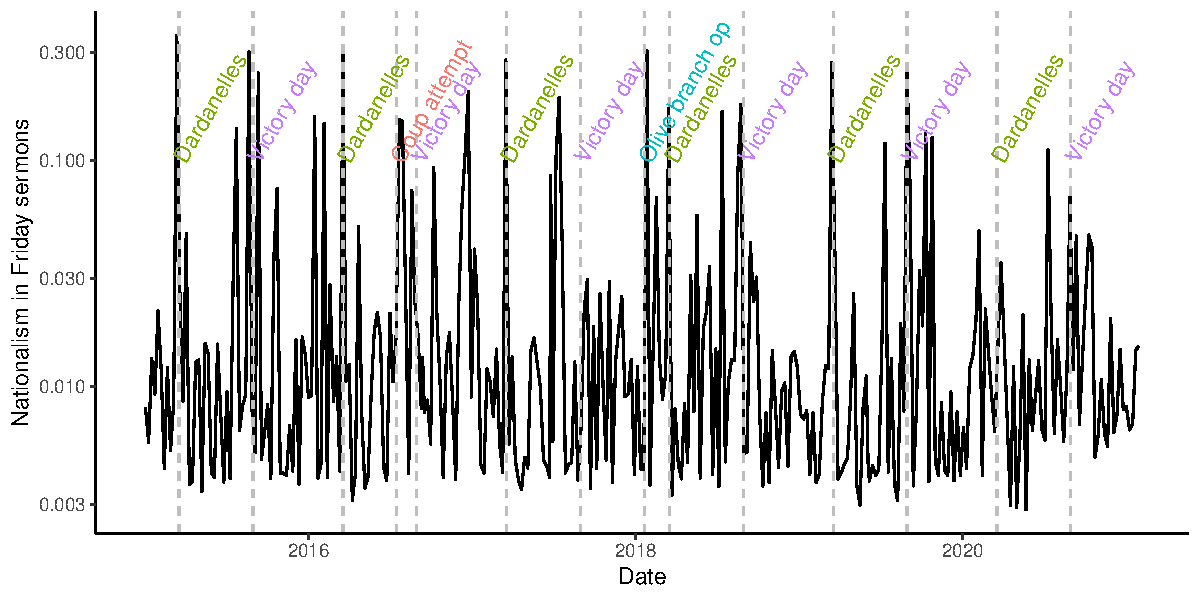
\includegraphics{Khutbas_files/figure-latex/fig-3-1} 

}

\caption{Nationalism (topic probability) in Friday khutbas and days of national importance.}\label{fig:fig-3}
\end{figure}

During the first several decades of the Turkish republic, which was founded in 1923, the Galippoli campaign was not regarded as a significant part of national identity (Uyar \protect\hyperlink{ref-uyar2016remembering}{2016}). In fact, for the founding elite the war of independence that took place after WWI that lead to the foundation of Turkey in 1923 was much more significant. The AKP government, however, mobilised a publicity campaign and a memorialisation project around the Dardanelles victory (Uyar \protect\hyperlink{ref-uyar2016remembering}{2016}). The Battle of Dardanelles is important for AKP because it signals an emphasis on the pre-republican Ottoman era, and as such Turkey's influence beyond the current borders, as well as the religious character of the pre-republic war. I quote below parts of a sermon from March 2019 which demonstrates the significance of Dardanelles for TPRA. The sermon celebrates martyrdom for the ``sake of religion, homeland, nation, state, and freedom'', places the event on a centuries long religious struggle, and uses it to boost nationalism today and for future generations.

\begin{quote}
``THE TURKISH VICTORY OF THE BATTLE OF GALLIPOLI AND THE ESPRIT DE CORPS. \ldots{} Honorable Believers! The martyrdom, the name for giving souls for the sake of holy values ordered by Allah (s.w.t.) to be protected, is one of the most supreme positions since a martyr takes the risk of abandoning all such beloved ones as his mother, father, wife, and children for the sake of religion, homeland, nation, state, and freedom. \ldots{} For centuries, our ancestors have protected the lands we live on through their faith in Allah (s.w.t.), their love for homeland, their courage, and sacrifice. \ldots{} Dear Believers!
Today, what falls upon us is to comprehend the magnificent spirit having reared in Çanakkale {[}Dardanelles{]}, to gather around our values that make us `us', and the nation that we are, and to transfer them to our next generations'' (TPRA, Friday khutba, 15.03.2019).
\end{quote}

It is also remarkable that we do not observe nationalism in TPRA's sermons on the Turkish national day (29 October) which marks the foundation of Turkish Republic. 29 October is arguably the most important date for the founding elite. Instead, the Victory Day (30 August) which commemorates the decisive victory of the Turkish forces in the Greco-Turkish war in 1922, seems to be more important for TPRA.

Figure \ref{fig:fig-3} also shows that nationalism in sermons also spikes as a response to serious threats the government faces (Alper et al. \protect\hyperlink{ref-alper2020changes}{2020}). The multiple spikes after the coup attempt on 15 July 2016 are notable. The coup attempt came as a result of a power struggle between the AKP and other Islamist factions, most notably Gulenists, after dismantling the old secular establishment (Esen and Gumuscu \protect\hyperlink{ref-esen2017turkey}{2017}). The attempt which was mainly concentrated in Ankara and Istanbul failed promptly. AKP utilised heavily TPRA's organisational reach in mobilising anti-coup demonstrations (Esen and Gumuscu \protect\hyperlink{ref-esen2017turkey}{2017}). On the night of the coup, TPRA orderd nearly 90,000 mosques in the country to cite the salah prayer as a call to defend the government on religious grounds. The mosques' role in anti-coup protests was crucial in overturning the attempt (Ünver and Alassaad \protect\hyperlink{ref-unver2016turks}{2016}). In fact, in the history of Turkey mosques have never played as much of a visible role as on the night of the coup attempt (Esen and Gumuscu \protect\hyperlink{ref-esen2017turkey}{2017}). I paste below selected parts of the sermon that came right after the coup attempt. The structure is similar as the one above. The sermon places the event in a centuries old struggle and aims to bolster unity and nationalism.

\begin{quote}
``Dear Brothers and Sisters! On the night of July 15, we went through one of the longest and darkest nights in our nation's history. Lord Almighty granted our nation to stand together with all its segments and we protected what has been entrusted to us. \ldots{} These treacherous attacks also showed this: Those who attempt to repress and defame our glorious nation are doomed to be humiliated and abominated! \ldots{} Esteemed Brothers and Sisters! Infinite thanks to Allah that this country has been a home for Muslims for centuries. This nation is the children of martyrs. \ldots{} O Allah. Save us from all enemies, from within and outside, who may undermine the survival of our state and our nation! \ldots{}'' (TPRA, Friday khutba, 22.07.2016)
\end{quote}

TPRA adressess significant threats to the state and government in other areas too. Figure \ref{fig:fig-4} shows the topics health and patience in the sermons over time. The Covid-19 pandemic started at the end of 2019 but the surge in health and patience in sermons corresponds with the first governmental restrictions (the first lockdown) on 15.03.2020. I translate below parts of the sermons that came right before and after the first lockdown. The sermons include practical tips and public health messages. They also offer solace in religion and God.

\begin{quote}
``PRECAUTION IS ON MUSLIMS, JUDGEMENT IS FROM ALLAH. Honorable Muslims! During the history, many diseases have been cured with Allah's help and humans' effort. God willing, a cure will also be found for the Coronavirus which has been spread all over the world. \ldots{} To protect ourselves, we should keep ourselves, our clothes, food, and environment clean. \ldots{} God entrusts our health to us. Muslims' duty is to honour this trust. In doing so, with God's help we obtain peace. We find cure for our troubles and diseases\ldots.'' (TPRA, Friday khutba, 13.03.2020)
\end{quote}

\begin{quote}
``BELIEVER DURING HARDSHIP. Honorable Muslims! Humanity is going through a difficult time. \ldots{} May Allah (s.w.t.) have mercy on those who lost their lives, may their families find peace, may patients find cure. \ldots{} One of our most important duties during this outbreak is complying with the directives of authorities. \ldots{} Of course, everything happens within God's power, wisdom, and knowledge. But humans' weaknesses and ambition have played an important role in this trouble. \ldots{} Crossing the borders drawn by God is leading humanity to disaster. \ldots{} Another duty of us is to keep our discernment and resilience. \ldots{} Most important means that will give us strength and assurance are taking refuge in God and putting ourselves in God's hands\ldots.'' (TPRA, Friday khutba, 27.03.2020)
\end{quote}

\begin{figure}

{\centering 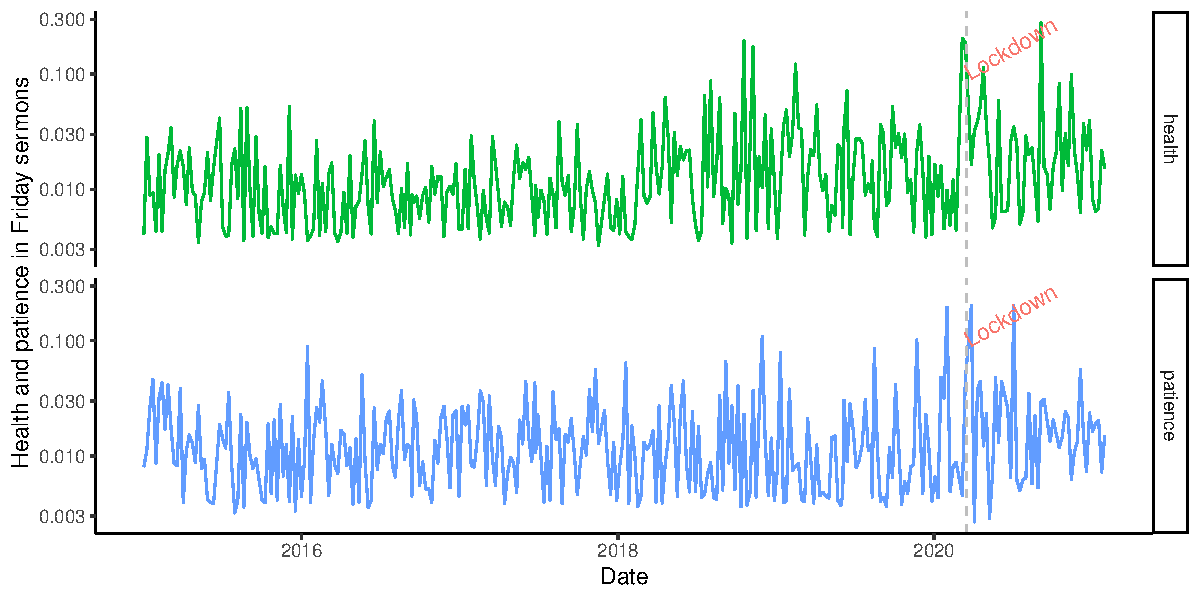
\includegraphics{Khutbas_files/figure-latex/fig-4-1} 

}

\caption{Health and patience (topic probability) in Friday khutbas and the pandemic.}\label{fig:fig-4}
\end{figure}

For completeness, Figure \ref{fig:fig-5} shows the topics business, family, and trust in sermons over time. Due to space restrictions, I will not be discussing the sermons on these topics in detail. One exception is the topic business, which seems to have become more salient after 2017. Interestingly, Turkey's Gross Domestic Product growth has started to decline during this time. GDP growth was 7.5 percent in 2017 which dropped to 0.9 percent by 2019. This period also corresponds with a surge in interests rates which were stable around 8 percent in 2017, shooting up to 24 percent by the summer of 2019. The sermon in August 2019 addresses this issue, as I quote below.

\begin{quote}
``SOCIAL HARMS OF INTEREST \ldots{} Dear Muslims! Islam declares all kinds of interest as haram definitely. It considers the operations with interest as one of the greatest sins. \ldots{} Interest decreases the baraqah of not only the property but also the life. Interest cause many bankruptcies suicides, dissolution of families, and wasted lives. \ldots{} Then, let us stay away from the disaster of interest which has been one the biggest means of exploitation and oppression in economic life throughout the history. \ldots{} In this temporary world life, let us try to earn
halal money\ldots{}'' (TPRA, Friday khutba, 23.08.2019)
\end{quote}

\begin{figure}

{\centering 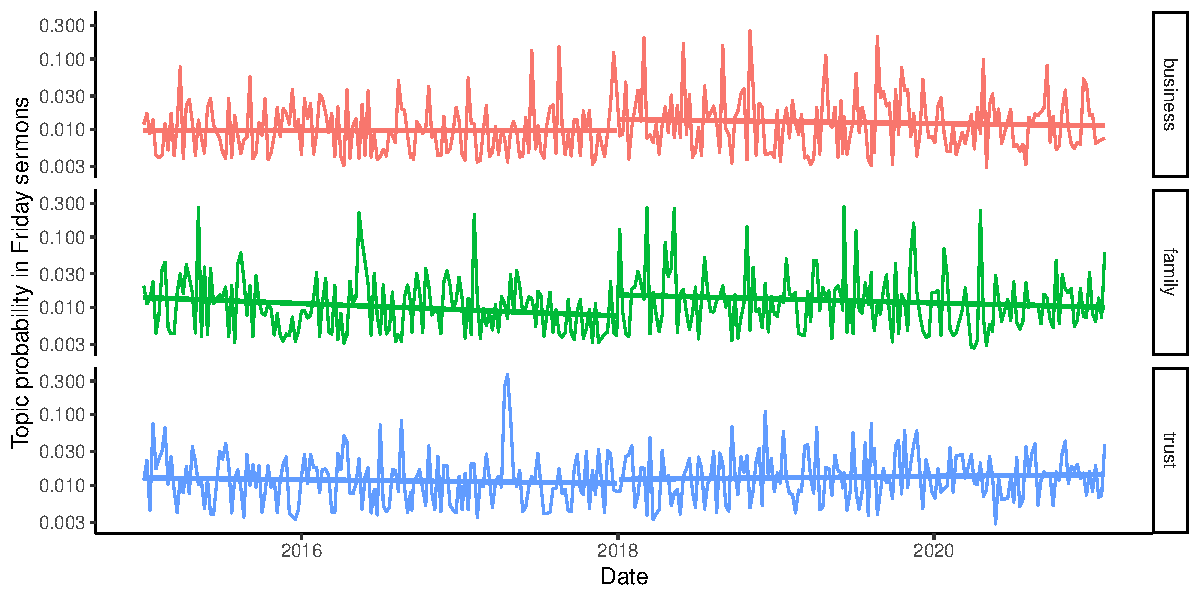
\includegraphics{Khutbas_files/figure-latex/fig-5-1} 

}

\caption{Family, trust, and businness (topic probability) in Friday khutbas. Linear trends before and after 2018 are added.}\label{fig:fig-5}
\end{figure}

The analysis above shows that the sermons written by TPRA respond to economic, security, and public health threats the country faces. The sermons aim to alleviate negative effects of shocks, offer solace in religion during hardships, and bolster nationalism, unity, and obedience. In the next section, I will discuss whether these sermons affect social media behaviour.

\hypertarget{tweets}{%
\subsection{Tweets}\label{tweets}}

Figure \ref{fig:fig-6} shows the weekly number of tweets in each of the six topic over time. Throughout all analyses, a week is constructed to run from Friday to next Thursday, in keeping with the fact that the sermons take place on Fridays. Nationalism, again, appears as one of the most prevalent Twitter topics among the ones sampled here. The increase in tweets on health and patience following the first Covid lockdown in March 2020 is notable. Figure \ref{fig:fig-7} shows the associations between the prevalence of a topic in a sermon, and the number of tweets on that topic in the week following the sermon. Generally, a positive association is observed between tweets on a topic and the sermon topic probability.

\begin{figure}
\centering
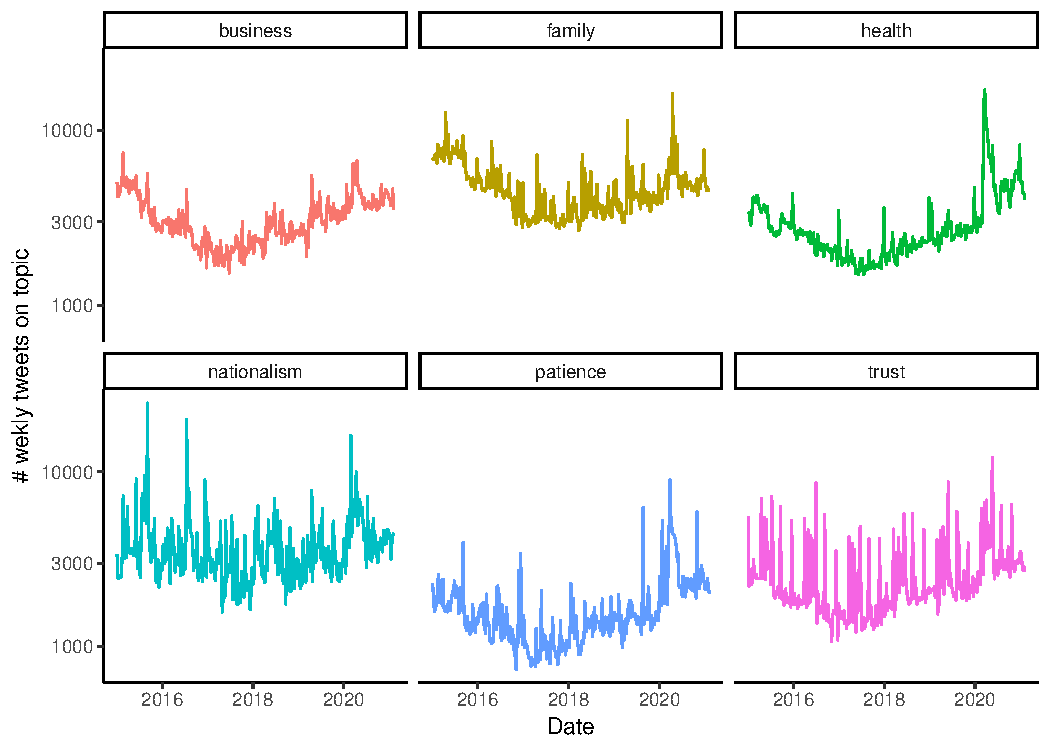
\includegraphics{Khutbas_files/figure-latex/Tweets.pdf}
\caption{\label{fig:fig-6}Weekly number of tweets per topic over time.}
\end{figure}

\begin{figure}

{\centering 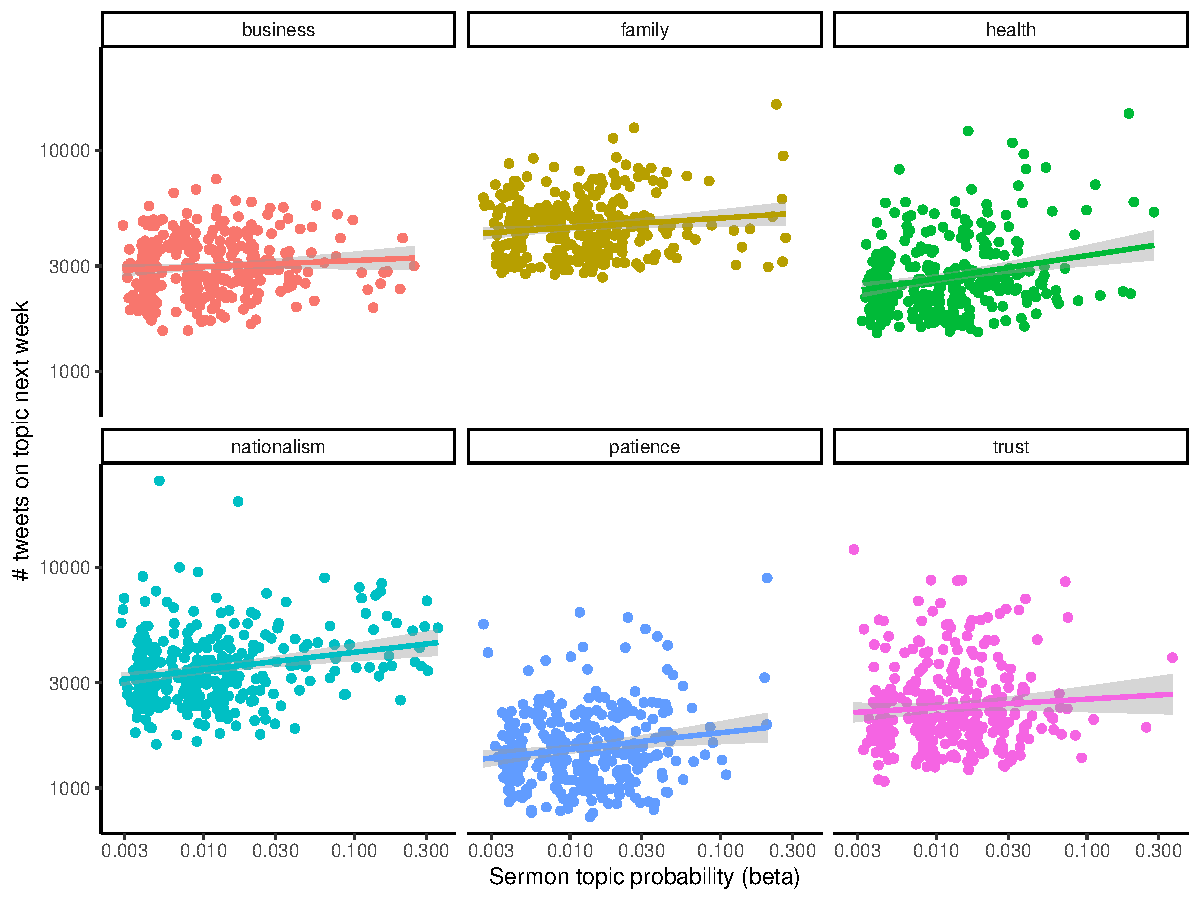
\includegraphics{Khutbas_files/figure-latex/fig-7-1} 

}

\caption{Tweets versus Friday sermon topics.}\label{fig:fig-7}
\end{figure}

Note, however, that there might be confounders that affect both the sermon content and tweets. For example, if a week contains, say the aniversary of the battle of Dardanelles (18 March), that week's sermon may have a more nationalist tone, while people, independently of the sermon, may tweet more nationalistically in that week too. To address these potential confounders which would render the associations in Figure \ref{fig:fig-7} spurious, I fit the following quasi-Poisson regression model that predicts \(N_{td}\) which is the number of tweets on topic \(t = 1,..,6\) on week \(d = 2015/01/02,...,2021/02/05\):

\begin{equation}
log(E(N_{td})) = \theta_{0t} + \theta_{1t}\times beta_{td} + \theta_{2}N_{td-1} + \alpha_d \label{eq:poisson}
\end{equation}

In equation \eqref{eq:poisson}, \(\theta_{0t}\) is the topic specific intercept, \(\theta_{1t}\) is the topic specific coefficient for sermon topic probability \(beta\), \(\theta_2\) is the coefficient for the number of tweets on topic \(t\) in previous week (capturing path dependency in Twitter trends), and \(\alpha_d\) is the week ``fixed effects''. \(\alpha_d\) absorbs week-specific events (e.g.~Dardanelles, Victory Day, or Mother's Day corresponding to a week). While those week fixed effects control for all observed or unobserved confounders that are constant in a week but may vary week-to-week, they may not account fully for events that happen exactly on Fridays. Hence, I fit a second version of the model in equation \eqref{eq:poisson} whereby I restrict \(N_{td}\) to tweets that are tweeted only on Fridays pm, controlling for tweets tweeted on Fridays am (\(N_{td-1}\)).

\begin{figure}

{\centering 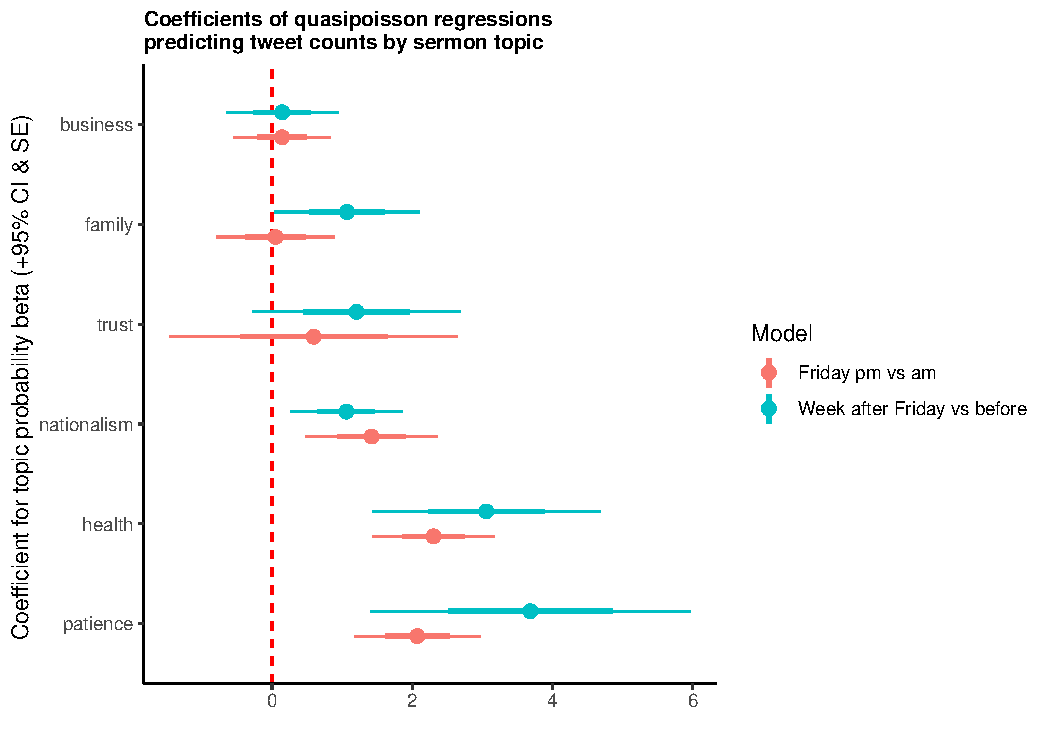
\includegraphics{Khutbas_files/figure-latex/fig-8-1} 

}

\caption{Coefficients of quasipoisson regressions predicting tweet counts by sermon topic. Coefficients are adjusted for week fixed effects, sermon topic fixed effects, and tweet counts before the sermon (i.e tweet counts on the previous week or Friday a.m. depending on the model). Standard errors are clustered by week.}\label{fig:fig-8}
\end{figure}

Figure \ref{fig:fig-8} displays \(\theta_{1t}\), the estimated topic specific coefficients for sermon topic probability in the two versions of the model: (1) predicting tweets in the week after the sermon while controlling for tweets before the sermon and (2) predicting tweets on Friday pm while controlling for tweets on Friday am. Figure \ref{fig:fig-8} indeed shows a generally positive effect of sermon topic on tweets. The effects are particularly strong and statistically significant for topics \emph{nationalism}, \emph{health}, and \emph{patience}. The effects for \emph{family} and \emph{trust}, too, are sizeable, though turns statistically insignificant when the analyis is restricted to tweets tweeted only on Fridays.

The estimated effects are generally large. For example, a 0.3 points increase in topic probability of health in a Friday sermon is predicted to double the number of tweets on health (\(\exp(2.3 \times 0.3)=1.99\)---taking the conservative Friday pm vs am point estimate). There are on average \textasciitilde3,000 weekly tweets on health, so this would result in 3,000 additional tweets on health. If we take the less conservative point estimate (the week after the sermon versus before), the excess number of health tweets due to the sermon increases to 4,500 (\(\exp(3.9 \times 0.3)=2.5 \rightarrow 3,000 \times 2.5 - 3,000 = 4,500\)). Figure \ref{fig:fig-8} also shows that the effect of sermons on tweets is not universal. For example, the effect of the sermon topic on tweets for business is small and statistically insignificant.

These results in Figure \ref{fig:fig-8} are robust to not including week fixed effects, not controlling for tweets before the sermon, and using the proportion of tweets on a topic rather than the number of tweets.

Before I move on to discussion and conclusions, I include below three anonymised (and translated) tweets. These tweets are on nationalism, health, and patience; the three topics for which the sermons are found to have the strongest effect. The examples below are tweeted right after a Friday sermon which strongly featured the same topic as the tweet exemplifies. Note that these are not necesarily representative of the tweets on the same topic (recall that the total number of tweets this study is based on is over 4 million). Nevertheless, they give an idea as to what type of tweets the sermons may be influencing. For example, the similarity between the tweet on nationalism and the sections of the sermon from the same date quoted above is remarkable.

\begin{quote}
\textbf{Nationalism:} ``Hail to all hearts who, on this holy Friday, said AMEN for the survival of this nation and our state. May you have a holy Friday.'' (tweeted on 2016-07-22, 14:10)
\end{quote}

\begin{quote}
\textbf{Health:} ``The greatest blessing is health, the most beautiful prayer is the one we say for our Muslim brothers.'' (tweeted on 2020-03-13, 14:35)
\end{quote}

\begin{quote}
\textbf{Patience:} ``Believers! Seek help in patience and in Prayer, Allah is with those that are patient (Baqarah 153). May Allah's mercy and blessings be upon us. May our Friday be blessed. \#HappyFriday'' (tweeted on 2020-07-03, 12:35)
\end{quote}

\hypertarget{discussion-and-conclusions}{%
\section{Discussion and Conclusions}\label{discussion-and-conclusions}}

In this study, I first analyse through machine learning the content of all Friday khutbas (sermons) written by the Turkish Presidency of Religious Affairs (TPRA) and read in thousands of mosques between January 2015 to February 2021 to millions of citizens. I focus on six topics of sociological interest: \emph{nationalism}, \emph{health}, \emph{patience}, \emph{trust}, \emph{business}, and \emph{family}. I find that the khutbas respond strongly to events of national importance and to the threats the government and the country face. Nationalism in sermons, for example, spikes regularly during the anniversaries of the Dardanelles victory which is a significant date for the ideology of the ruling cadre. Nationalism in sermons also spikes as a response to significant security threats, such as the coup attempt or Turkey's offensive in Syria. Similarly, health and patience feature strongly in sermons during and after the Covid-19 lockdown.

I then link the khutbas with over 4 millon tweets tweeted on the six selected topics between January 2015 and February 2021 to analyze whether the sermons affect behavior on Twitter. I find strong and significant effects of the content of the khutba on tweets, particularly for topics \emph{nationalism}, \emph{health}, and \emph{patience}. I also find that the effects of khutbas on tweets is not universal, for example, the effect for topic \emph{business} is small and statistically insignificant. Overall, these results show that TPRA is influential in shaping the public's social media content and that this influence is mainly prevalent on salient issues. More generally, these results show that mass religious activity can have strong effects on social media behavior.

This study aims to make a contribution in four fronts. The first one is to contribute to a debate on how religion and politics interact in Turkey. Since 2010, the Turkish government invests strongly in religious institutions, in line with an aim of raising a ``pious generation''. In this process, as some argue, TPRA has turned into a state apparatus imposing the political ideology of the ruling elite. It has been unclear, however, if TPRA has been influential in shaping public values and attitudes. Despite TPRA's very generous resources, individual religiosity has been in decline. Does this mean that the Turkish government's heavy investment in religion has not paid off? I here show that TPRA has indeed been influential, particularly on pressing and salient issues. Moreover, I document this influence in a domain which is arguably rather distant from the Mosque, namely in the digital world. One may expect this influence to be even stronger in the offline world where TPRA has been traditionally present, such as in Mosques, Quran courses, and many other events and projects TPRA organises. Hence, overall, it seems that money spent on TPRA is well spent from the government's perspective.

Secondly, the article makes a methodological contribution. The rise of ``computational social science'' offers opportunities to address long standing sociological questions in novel ways. Applications, however, tend to be restricted to traditionally quantitative topics and Western contexts. Here I apply these tools to analyse hundreds of sermons and millions of tweets, hopefully pushing the boundary of computational social science to the study of religion and politics in a non-Western context. Nevertheless, there is room for improvement in future research. In this study, I restrict the analysis to only selected topics for space restrictions and a limited time frame for data constraints. Future research can extend this study in various ways. For example, one can focus exclusively on khutbas and study the evolution of the broader set of sermons topics over time.

Thirdly, the article contributes to the long standing debate on the interplay between politics and religion. Classical theorists from Durkheim to Marx investigate the link between religion and society. The ``opiate'' argument of Marx in particular is rather well known. Much empirical research that tests this argument focuses on how individuals respond to various forms of shocks and whether individual religiosity buffers these shocks. How religious institutions respond to these shocks is relatively understudied, perhaps because of lack of survey data on institutions. I find through analysing the sermons that the religious authority of the country indeed aims to alleviate the detrimental effects of shocks, offering peace and solace in religion. Moreover, it aims to bolster nationalism, unity, and obedience. These messages in sermons also seem to find their way, as indicated by an influence on Twitter.

Finally, the results are relevant for the debate on secularisation. The secularisation theory predicts a nearly universal transition from religious to nonreligious as countries modernise. There is support for such a trend, but evidence is mostly from the West. Turkey may be seen as a challenge for this theory, for it was traditionally a secular country but embodies a recent rise of political Islam. Yet, as I show above individual religiosity is still in decline. What makes this decline particularly remarkable is that it happens in spite of the heavy top-down investment in religion \emph{and} of the effectiveness of the religious authority in shaping public's behaviour as I document using Twitter. The Turkish case may shows that top-down investment in religion may slow down secularisation--one would indeed expect religiosity to plummet without the governmental investment--but not reverse it. Turkish government's aim of raising a pious generation thus seems to be an uphill battle.

\hypertarget{references}{%
\section{References}\label{references}}

\linespread{1}

\hypertarget{refs}{}
\leavevmode\hypertarget{ref-aksoy2020religiosity}{}%
Aksoy, Ozan, David Bann, Meg E. Fluharty, and Alita Nandi. 2021. ``Religiosity and Mental Wellbeing Among Members of Majority and Minority Religions: Findings from Understanding Society, the Uk Household Longitudinal Study.'' \emph{American Journal of Epidemiology}.

\leavevmode\hypertarget{ref-aksoy2018political}{}%
Aksoy, Ozan and Francesco C. Billari. 2018. ``Political Islam, Marriage, and Fertility: Evidence from a Natural Experiment.'' \emph{American Journal of Sociology} 123(5):1296--1340.

\leavevmode\hypertarget{ref-AG21}{}%
Aksoy, Ozan and Diego Gambetta. 2021. ``The Politics Behind the Veil.'' \emph{European Sociological Review} 37(1):67--88.

\leavevmode\hypertarget{ref-alper2020changes}{}%
Alper, Sinan, Fatih Bayrak, Elif Öykü Us, and Onurcan Yilmaz. 2020. ``Do Changes in Threat Salience Predict the Moral Content of Sermons? The Case of Friday Khutbas in Turkey.'' \emph{European Journal of Social Psychology} 50(3):662--72.

\leavevmode\hypertarget{ref-bail2017channeling}{}%
Bail, Christopher A., Taylor W. Brown, and Marcus Mann. 2017. ``Channeling Hearts and Minds: Advocacy Organizations, Cognitive-Emotional Currents, and Public Conversation.'' \emph{American Sociological Review} 82(6):1188--1213.

\leavevmode\hypertarget{ref-bauer2020writing}{}%
Bauer, Paul C. 2020. ``Writing a Reproducible Paper in R Markdown.'' \emph{SSRN Electronic Journal} 8.

\leavevmode\hypertarget{ref-becker2013not}{}%
Becker, Sascha O. and Ludger Woessmann. 2013. ``Not the Opium of the People: Income and Secularization in a Panel of Prussian Counties.'' \emph{American Economic Review} 103(3):539--44.

\leavevmode\hypertarget{ref-blei2003latent}{}%
Blei, David M., Andrew Y. Ng, and Michael I. Jordan. 2003. ``Latent Dirichlet Allocation.'' \emph{The Journal of Machine Learning Research} 3:993--1022.

\leavevmode\hypertarget{ref-bruce2011sec}{}%
Bruce, Steve. 2011. \emph{Secularization: In Defence of an Unfashionable Theory}. Oxford: Oxford University Press.

\leavevmode\hypertarget{ref-bulut2017mediatized}{}%
Bulut, Ergin and Erdem Yörük. 2017. ``Mediatized Populisms\textbar{} Digital Populism: Trolls and Political Polarization of Twitter in Turkey.'' \emph{International Journal of Communication} 11:25.

\leavevmode\hypertarget{ref-chen2010club}{}%
Chen, Daniel L. 2010. ``Club Goods and Group Identity: Evidence from Islamic Resurgence During the Indonesian Financial Crisis.'' \emph{Journal of Political Economy} 118(2):300--354.

\leavevmode\hypertarget{ref-durkheim1965elementary}{}%
Durkheim, Emile. 1965. \emph{The Elementary Forms of the Religious Life {[}1912{]}}. New York: Free Press.

\leavevmode\hypertarget{ref-compsocsciARS20}{}%
Edelmann, Achim, Tom Wolff, Danielle Montagne, and Christopher A. Bail. 2020. ``Computational Social Science and Sociology.'' \emph{Annual Review of Sociology} 46(1):61--81.

\leavevmode\hypertarget{ref-esen2017turkey}{}%
Esen, Berk and Sebnem Gumuscu. 2017. ``Turkey: How the Coup Failed.'' \emph{Journal of Democracy} 28(1):59--73.

\leavevmode\hypertarget{ref-Guxf6zaydin2008}{}%
Gözaydin, İştar. 2008. ``Religion, Politics, and the Politics of Religion in Turkey.'' Pp. 159--76 in \emph{Religion, politics, and turkey's eu accession}, edited by D. Jung and C. Raudvere. New York: Palgrave Macmillan US.

\leavevmode\hypertarget{ref-grimmer2013text}{}%
Grimmer, Justin and Brandon M. Stewart. 2013. ``Text as Data: The Promise and Pitfalls of Automatic Content Analysis Methods for Political Texts.'' \emph{Political Analysis} 21(3):267--97.

\leavevmode\hypertarget{ref-Hac14}{}%
Hacettepe University Institute of Population Studies. 2014. \emph{2003-2013 Turkey Demographic and Health Survey}. Ankara, Turkey: Hacettepe University Institute of Population Studies, T.R. Ministry of Development; TÜBİTAK.

\leavevmode\hypertarget{ref-isman2018diffusion}{}%
Isman, Aytekin and Engin Dagdeviren. 2018. ``Diffusion of Twitter in Turkey.'' \emph{Turkish Online Journal of Educational Technology-TOJET} 17(4):1--7.

\leavevmode\hypertarget{ref-Racialized}{}%
Kennedy, Ian, Chris Hess, Amandalynne Paullada, and Sarah Chasins. 2020. ``Racialized Discourse in Seattle Rental Ad Texts.'' \emph{Social Forces} 99(4):1432--56.

\leavevmode\hypertarget{ref-Kon19}{}%
KONDA. 2019a. ``2018 Hayat Tarzlari {[}Lifestyles in 2018{]}.'' \emph{Report, Url: Https://Bit.ly/3uRZRCk}.

\leavevmode\hypertarget{ref-Kon19rap}{}%
KONDA. 2019b. ``TÜRKİYE'DE Toplumsal Cinsiyet Raporu {[}Gender in Turkey{]}.'' \emph{Report, Url: Https://Bit.ly/32DRT33}.

\leavevmode\hypertarget{ref-kuran2018islam}{}%
Kuran, Timur. 2018. ``Islam and Economic Performance: Historical and Contemporary Links.'' \emph{Journal of Economic Literature} 56(4):1292--1359.

\leavevmode\hypertarget{ref-Lazer1060}{}%
Lazer, David M. J., Alex Pentland, Duncan J. Watts, Sinan Aral, Susan Athey, Noshir Contractor, Deen Freelon, Sandra Gonzalez-Bailon, Gary King, Helen Margetts, Alondra Nelson, Matthew J. Salganik, Markus Strohmaier, Alessandro Vespignani, and Claudia Wagner. 2020. ``Computational Social Science: Obstacles and Opportunities.'' \emph{Science} 369(6507):1060--2.

\leavevmode\hypertarget{ref-light2017managing}{}%
Light, Ryan and Colin Odden. 2017. ``Managing the Boundaries of Taste: Culture, Valuation, and Computational Social Science.'' \emph{Social Forces} 96(2):877--908.

\leavevmode\hypertarget{ref-marx1970marx}{}%
Marx, Karl. 1970. \emph{Marx's Critique of Hegel's Philosophy of Right}. Cambridge: Cambridge University Press.

\leavevmode\hypertarget{ref-mcfarland2013differentiating}{}%
McFarland, Daniel A., Daniel Ramage, Jason Chuang, Jeffrey Heer, Christopher D. Manning, and Daniel Jurafsky. 2013. ``Differentiating Language Usage Through Topic Models.'' \emph{Poetics} 41(6):607--25.

\leavevmode\hypertarget{ref-mecham2004ashes}{}%
Mecham, R. Quinn. 2004. ``From the Ashes of Virtue, a Promise of Light: The Transformation of Political Islam in Turkey.'' \emph{Third World Quarterly} 25(2):339--58.

\leavevmode\hypertarget{ref-Munger_Guess_Hargittai_2021}{}%
Munger, Kevin, Andrew M. Guess, and Eszter Hargittai. 2021. ``Quantitative Description of Digital Media: A Modest Proposal to Disrupt Academic Publishing.'' \emph{Journal of Quantitative Description: Digital Media} 1.

\leavevmode\hypertarget{ref-nikita2016select}{}%
Nikita, Murzintcev. 2016. ``Select Number of Topics for Lda Model.'' \emph{Available on: Https://Cran. Rproject. Org/Web/Packages/Ldatuning/Vignettes/Topics. Html.{[}March 3rd, 2019{]}}.

\leavevmode\hypertarget{ref-norris2011sacred}{}%
Norris, Pippa and Ronald Inglehart. 2011. \emph{Sacred and Secular: Religion and Politics Worldwide}. Cambridge University Press.

\leavevmode\hypertarget{ref-ozbudun2006political}{}%
Özbudun, Ergun. 2006. ``From Political Islam to Conservative Democracy: The Case of the Justice and Development Party in Turkey.'' \emph{South European Society \& Politics} 11(3-4):543--57.

\leavevmode\hypertarget{ref-Ozt16}{}%
Öztürk, Ahmet Erdi. 2016. ``Turkey's Diyanet Under Akp Rule: From Protector to Imposer of State Ideology?'' \emph{Southeast European and Black Sea Studies} 16(4):619--35.

\leavevmode\hypertarget{ref-uxf6ztuxfcrk_suxf6zeri_2018}{}%
Öztürk, Ahmet Erdi and Semiha Sözeri. 2018. ``Diyanet as a Turkish Foreign Policy Tool: Evidence from the Netherlands and Bulgaria.'' \emph{Politics and Religion} 11(3):624--48.

\leavevmode\hypertarget{ref-roberts2014structural}{}%
Roberts, Margaret E., Brandon M. Stewart, Dustin Tingley, Christopher Lucas, Jetson Leder-Luis, Shana Kushner Gadarian, Bethany Albertson, and David G. Rand. 2014. ``Structural Topic Models for Open-Ended Survey Responses.'' \emph{American Journal of Political Science} 58(4):1064--82.

\leavevmode\hypertarget{ref-Sch21}{}%
Schnabel, Landon. 2020. ``Opiate of the Masses? Inequality, Religion, and Political Ideology in the United States.'' \emph{Social Forces} 99(3):979--1012.

\leavevmode\hypertarget{ref-schnabel2017persistent}{}%
Schnabel, Landon and Sean Bock. 2017. ``The Persistent and Exceptional Intensity of American Religion: A Response to Recent Research.'' \emph{Sociological Science} 4:686--700.

\leavevmode\hypertarget{ref-silge2017text}{}%
Silge, Julia and David Robinson. 2017. \emph{Text Mining with R: A Tidy Approach}. " O'Reilly Media, Inc.".

\leavevmode\hypertarget{ref-Sto20}{}%
Stolz, Jörg. 2020. ``Secularization Theories in the Twenty-First Century: Ideas, Evidence, and Problems. Presidential Address.'' \emph{Social Compass} 67(2):282--308.

\leavevmode\hypertarget{ref-tocqueville2003democracy}{}%
Tocqueville, Alexis. 2003. \emph{Democracy in America: And Two Essays on America {[}1835{]}}. London: Penguin.

\leavevmode\hypertarget{ref-uyar2016remembering}{}%
Uyar, Mesut. 2016. ``Remembering the Gallipoli Campaign: Turkish Official Military Historiography, War Memorials and Contested Ground.'' \emph{First World War Studies} 7(2):165--91.

\leavevmode\hypertarget{ref-unver2016turks}{}%
Ünver, H. Akın and Hassan Alassaad. 2016. ``How Turks Mobilized Against the Coup: The Power of the Mosque and the Hashtag.'' \emph{Foreign Affairs} 14.

\leavevmode\hypertarget{ref-voas2009rise}{}%
Voas, David. 2009. ``The Rise and Fall of Fuzzy Fidelity in Europe.'' \emph{European Sociological Review} 25(2):155--68.

\leavevmode\hypertarget{ref-voas2016united}{}%
Voas, David and Mark Chaves. 2016. ``Is the United States a Counterexample to the Secularization Thesis?'' \emph{American Journal of Sociology} 121(5):1517--56.

\leavevmode\hypertarget{ref-voas2018even}{}%
Voas, David and Mark Chaves. 2018. ``Even Intense Religiosity Is Declining in the United States: Comment.'' \emph{Sociological Science} 5:694--710.

\leavevmode\hypertarget{ref-WVB17}{}%
Welbers, Kasper, Wouter Van Atteveldt, and Kenneth Benoit. 2017. ``Text Analysis in R.'' \emph{Communication Methods and Measures} 11(4):245--65.

\clearpage

\appendix

\hypertarget{appendix}{%
\section{Appendix}\label{appendix}}

\hypertarget{sec:topnum}{%
\subsection{Selecting the number of topics in sermons}\label{sec:topnum}}

\begin{figure}
\centering
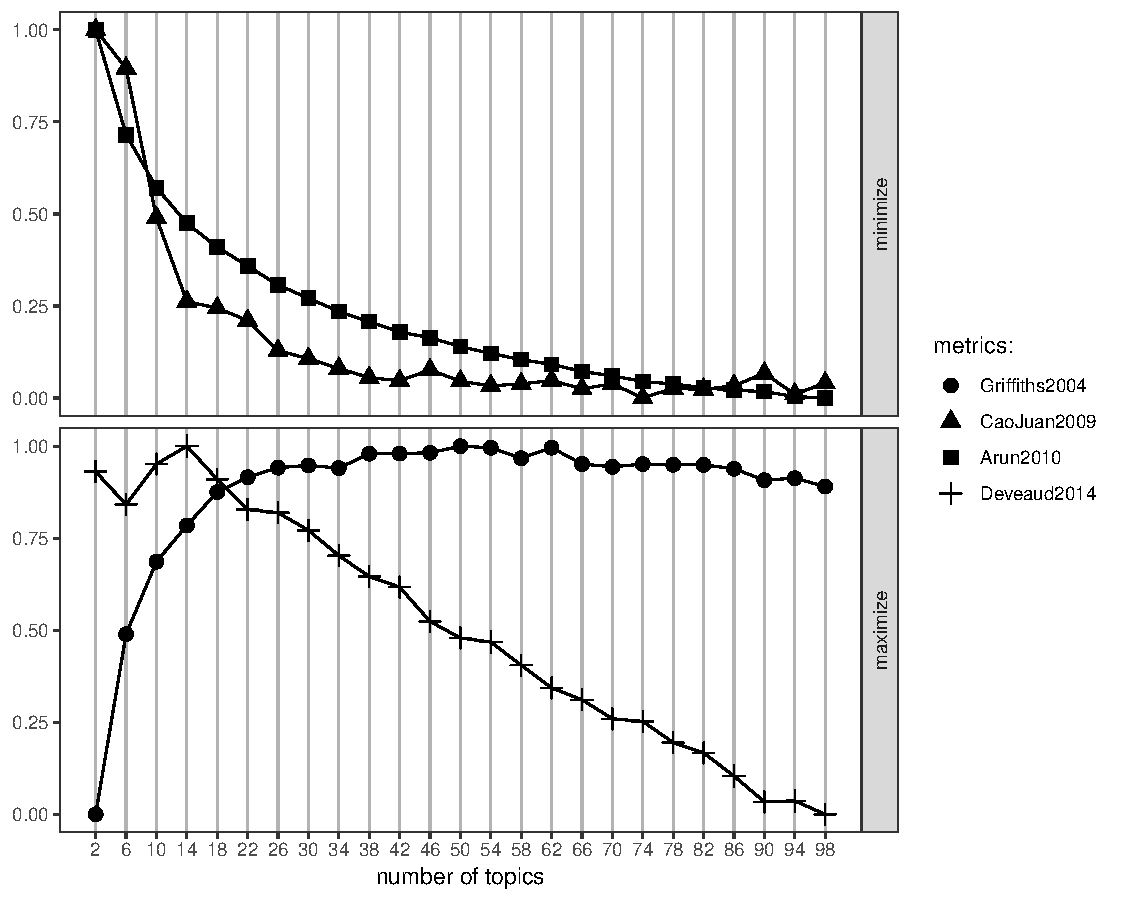
\includegraphics{Khutbas_files/figure-latex/number-topics.pdf}
\caption{\label{fig:unnamed-chunk-1}Fit statistics and the number of latent topics in sermons}
\end{figure}

\end{document}
